\section{Building Generation}

\begin{figure}[H]
  \centering

  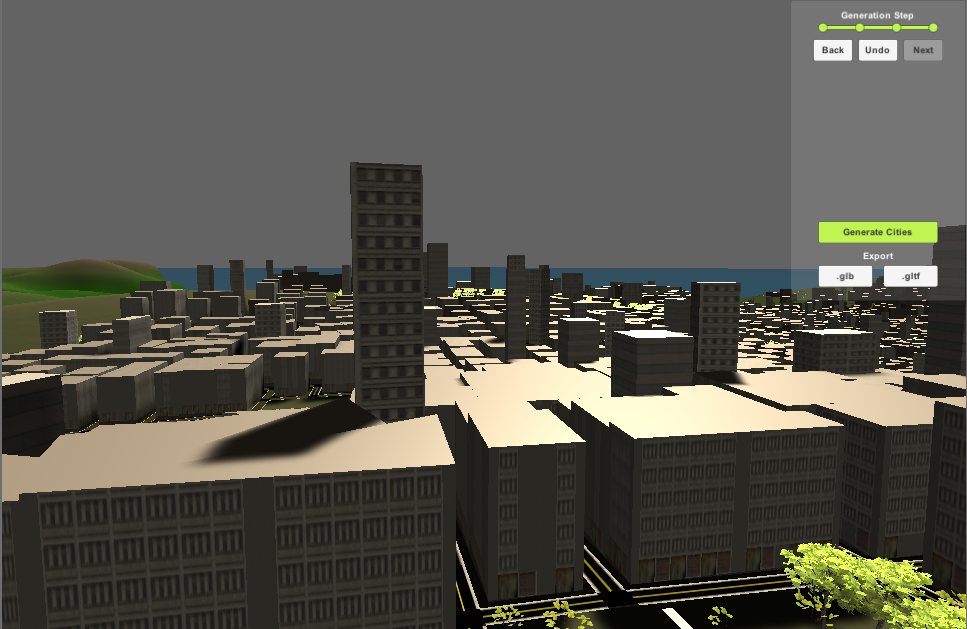
\includegraphics[width=0.7\textwidth]{figure/skyline.PNG}
  \caption{Skyline of \textit{Manhattan} and \textit{Skyscraper} buildings together.}

  \label{fig:skyline-result}
\end{figure}


The Building Generator creates buildings for the plots whose labels are \textit{Manhattan} or \textit{Skyscraper}. 
An example of a skyline with both \textit{Manhattan} and \textit{Skyscraper} can be seen in Figure \ref{fig:skyline-result}.
\textit{Manhattan} buildings are very versatile via the possibility to have different floor types L-systems and different wall segment L-systems. 
The final implementation had a single floor type generator called \textit{StraightManhattanFloorsGenerator (Straight)}. 
The name was derived from the possibility of having buildings that became smaller as the building grew higher. 
This was never implemented, though. 

\textit{Straight} can generate four different floor types: \textit{First}, \textit{Normal}, \textit{EveryOther}, and \textit{RepeatWindow}. 
An L-system is used to generate the floor types. The axiom is \textit{First} and one of \textit{Normal}, \textit{EveryOther}, or \textit{RepeatWindow}. 
The generation is quite simple. It just repeats one of the last three mentioned floor types until it has reached its desired height. 

The different floor types mentioned represent an L-system that generates some wall segments for the floor per walls. 
First can generate \textit{Corner}, \textit{ShopWindow}, \textit{Wall}, and \textit{Door}. \textit{Normal} can generate \textit{Corner}, \textit{Wall}, and \textit{Window}, but it only generates half of the wall. 
For the other half, it copies the first half and reverses it. \textit{EveryOther} can generate \textit{Corner}, \textit{Wall}, and \textit{Window}. 
It switches though between \textit{Wall} and \textit{Window}. The last floor type, \textit{RepeatWindow}, can only generate \textit{Corner} and \textit{Window}. 
It only has windows between the corners. An example of the generation of \textit{Straight}, with the four different floor types, can be found in Figure \ref{fig:wall-segment-generator}.


\begin{figure}[H]
  \centering

  \begin{subfigure}[b]{0.25\textwidth}
    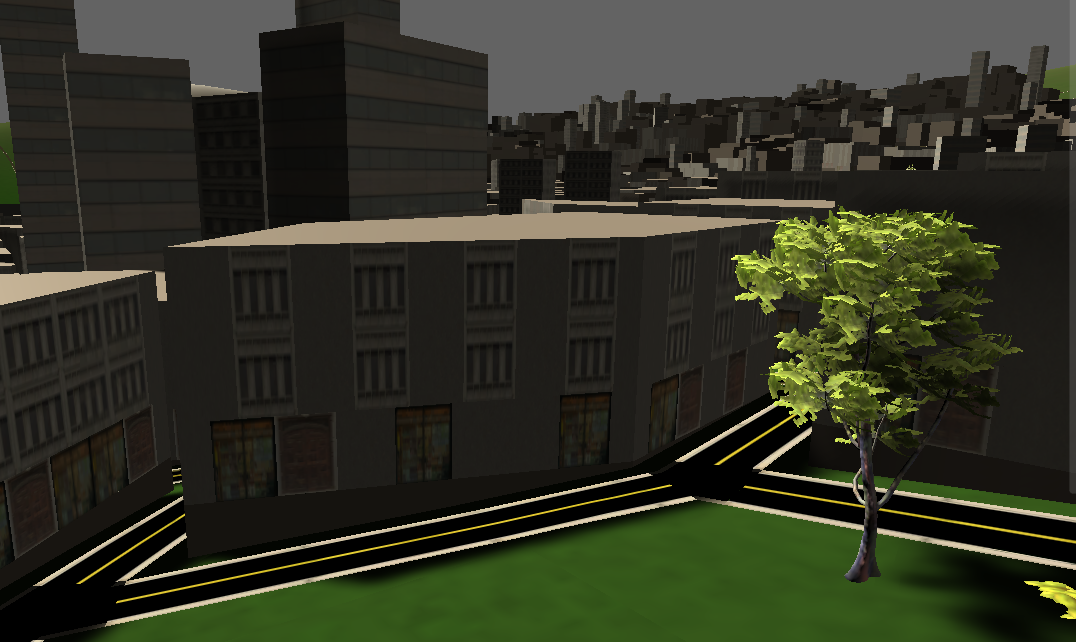
\includegraphics[width=\textwidth]{figure/building-every-other.PNG}
    \caption{\textit{EveryOtherFloor}.}
  \end{subfigure}
  \quad
  \begin{subfigure}[b]{0.25\textwidth}
    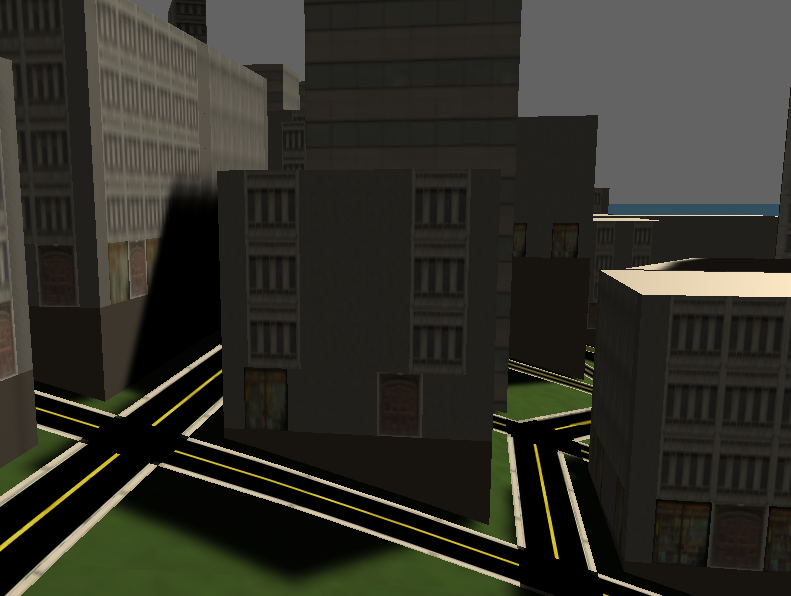
\includegraphics[width=\textwidth]{figure/building-normal.PNG}
    \caption{\textit{MirrorFloor}.}
  \end{subfigure}
  \quad
  \begin{subfigure}[b]{0.25\textwidth}
      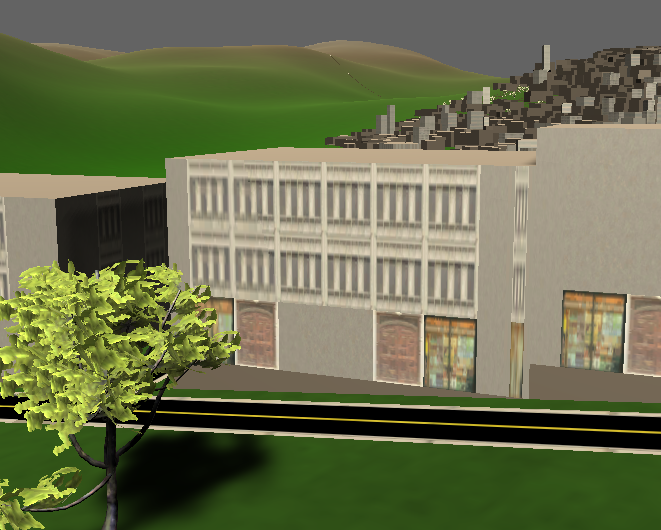
\includegraphics[width=\textwidth]{figure/building-only-window.PNG}
      \caption{\textit{OnlyWindowFloor}.}
  \end{subfigure}
  
  \caption{The three different wall segment generators. Notice that each building has a \textit{FirstFloor} wall segment generator on the first floor.}
  \label{fig:wall-segment-generator}
\end{figure}

Skyscraper has two different textures from which different sub-regions were sampled. In Figure \ref{fig:skyscraper-result}, you can see examples of them. 


  \begin{figure}[H]
    \centering
  
    \begin{subfigure}[b]{0.45\textwidth}
      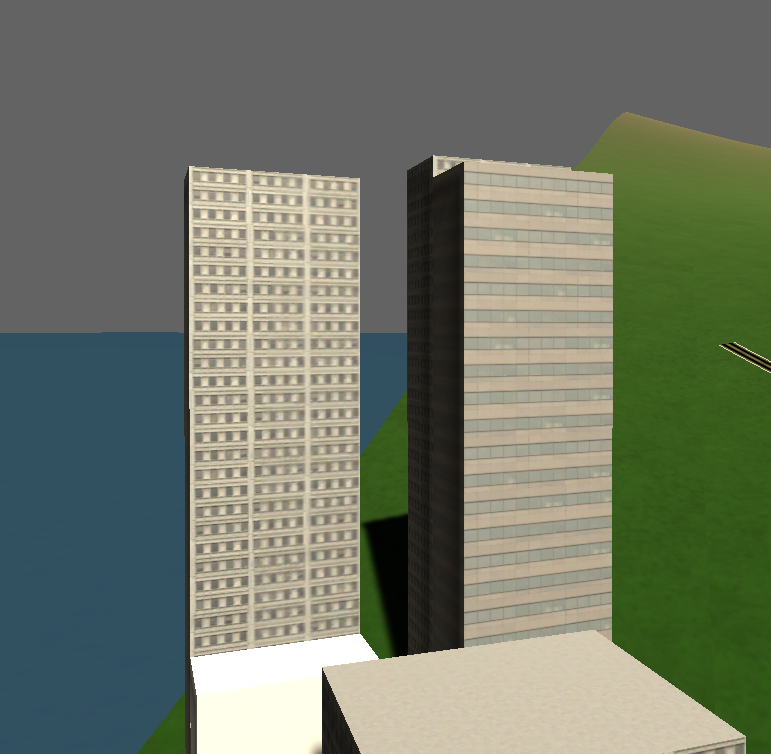
\includegraphics[width=\textwidth]{figure/skyscraper-close-up.PNG}
    \end{subfigure}
    \quad
    \begin{subfigure}[b]{0.45\textwidth}
      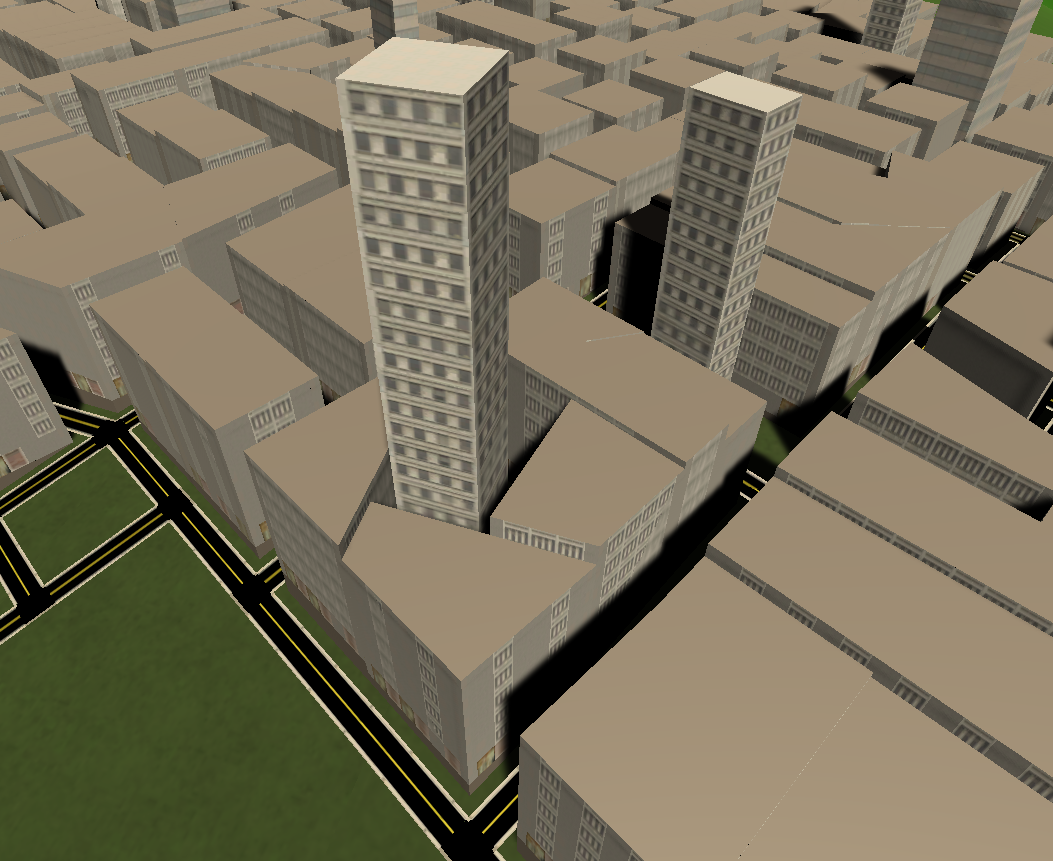
\includegraphics[width=\textwidth]{figure/wack.PNG}
    \end{subfigure}
    
    \caption{Various \texit{Skyscraper}s.}
    \label{fig:skyscraper-result}
  \end{figure}
 